\documentclass{article}
\usepackage{multicol,mwe}
\setlength{\columnsep}{1cm}

\usepackage{geometry}
 \geometry{
 total={160mm,230mm},
 top=20mm,
 }
 
 \usepackage{graphicx}
\graphicspath{ {./images/} }
 
\usepackage[backend=biber, sorting=none]{biblatex}
\addbibresource{references.bib}

\usepackage{amsmath, amsfonts, bm}
\usepackage{algorithm}
\usepackage[spaceRequire=false]{algpseudocodex}
\usepackage{appendix}
\usepackage{float}

\usepackage{xcolor}
\definecolor{codegreen}{rgb}{0,0.6,0}
\definecolor{codegray}{rgb}{0.5,0.5,0.5}
\definecolor{codepurple}{rgb}{0.28,0,0.52}
\definecolor{backcolour}{rgb}{0.95,0.95,0.95}

\usepackage{listings}
\usepackage{lmodern}
\ttfamily

\newcommand{\cbtt}[1]{\textcolor{codepurple}{\fontseries{b}\selectfont{\texttt{#1}}}}
\newcommand{\dbtt}[1]{\textcolor{codegreen}{\fontseries{b}\selectfont{\texttt{#1}}}}
\newcommand{\btt}[1]{{\fontseries{b}\selectfont{\texttt{#1}}}}

\lstdefinestyle{jsonstyle}{
    backgroundcolor=\color{backcolour},   
    commentstyle=\color{codegreen},
    keywordstyle=\color{magenta},
    numberstyle=\tiny\color{codegray},
    stringstyle=\color{codepurple},
    basicstyle=\tiny,
    breakatwhitespace=false,         
    breaklines=true,                 
    captionpos=b,                    
    keepspaces=true,                 
    numbers=left,                    
    numbersep=5pt,                  
    showspaces=false,                
    showstringspaces=false,
    showtabs=false,                  
    tabsize=1
}
\lstdefinestyle{pythonstyle}{
    backgroundcolor=\color{backcolour},   
    commentstyle=\color{codegreen},
    keywordstyle=\color{magenta},
    numberstyle=\tiny\color{codegray},
    stringstyle=\color{codepurple},
    basicstyle=\tiny,
    breakatwhitespace=false,         
    breaklines=true,                 
    captionpos=b,                    
    keepspaces=true,                 
    numbers=left,                    
    numbersep=5pt,                  
    showspaces=false,                
    showstringspaces=false,
    showtabs=false,                  
    tabsize=1
}


\title{Chromatography Model v 0.1}
\author{James Klimavicz}

\setcounter{tocdepth}{2}
 
\begin{document}

\maketitle
\section*{Overview}
The purpose of this package is to create realistic-looking chromatogram data, and then analyze the chromatograms to detect peaks, and calculate peak parameters for each peak. The package attempts to capture many qualities of authentic chromatograms. Key features include:

\begin{itemize}
\item Baselines noise, with the ability to reproduce some autoregressive behavior in the baseline signal, as expected for a time series.
\item Asymmetric peak shape, with peaks being modeled by exponentially-modified gaussian functions \cite{emg2}. Peaks that elute later tend to be broader and shorter, but with similar areas.
\item Solvent gradients and choices of solvent affect the baseline absorbance, and result in changes in the peak retention time of each compound. The change in retention time depends on the choice of solvents, percentage of each solvent, and the flow rate. 
\item Compound data for over 300 compounds, including UV-Vis data, have been pre-populated to produce random samples of various compounds. Samples can be defined with lists of compound names or CAS numbers
\item Ability to introduce small random variations in peak elution times and peak heights, both constant across an injection and also within an injection to produce realist variations between chromatograms for otherwise identical samples and methods.
\end{itemize}

%\begin{multicols}{2}
\tableofcontents


\section{Systems}\label{sec:sys}
Currently, a system is implemented to:
\begin{itemize}
\item store a system name,
\item allow for a system-specific deviation in retention time $\delta t_{\text{sys}}$, e.g. those due to differences in tubing lengths between column components, 
\item facilitate injections onto the column, and
\item allow for placing a new column with a different serial number into the system. 
\end{itemize}
The \cbtt{System} also stores any \texttt{**kwargs} provided to the class. Nothing is currently implemented for this, but this may be useful to have as a reference for, e.g., an output file.

\subsection{Columns}\label{sec:col}

The column itself is modeled by the \cbtt{Column} class, which keep track of injections, $n_{\text{inj}}$. Upon instantiation, the column is given attributes for column-specific differences for peak asymmetry $\delta A_{\text{def}}$, broadening $\delta B_{\text{def}}$, and retention time $\delta t_{\text{def}}$. 

It also contains an attribute for when a column may begin to fail, $n_{\text{fail}}$. After this number of injections is reached, each injection carries a probability of triggering a failure, equal to $0.00015 \cdot (n_{\text{inj}} - n_{\text{fail}})$. After failing, each injection causes slight increases in asymmetry $\delta A_{\text{fail}}$, broadening $\delta B_{\text{fail}}$, and retention times $\delta t_{\text{fail}}$, using the following formulas: 
\begin{align}
\rho &\in \text{Uniform}(0.95, 1.05)\nonumber \\
d &= n_{\text{inj}} - n_{\text{fail}} + 1 \nonumber \\
\xi &= 0.5 \rho \cdot \ln \left(1 + 10^{-7} \cdot \left(\frac{x}{2} -1 \right)^3 \right) \nonumber \\
\delta A_{\text{fail}} &= 20 \cdot \xi \cdot (A -1) \\
\delta B_{\text{fail}} &= \frac{\xi \cdot W}{20}  \\
\delta t_{\text{fail}} &= 1 + 0.01 \xi
\end{align}

When it then comes to a specific injection, the column parameters $\delta A_{\text{col}} = \delta A_{\text{def}} + \delta A_{\text{fail}}$, $\delta B_{\text{col}} = \delta B_{\text{def}} + \delta B_{\text{fail}}$, and $\delta t_{\text{col}} = \delta t_{\text{def}} + \delta t_{\text{fail}}$ are surfaced to adjust the appearance of the chromatogram.

\section{Methods}\label{sec:methods}
There are two types of methods: instrument methods, which determine how data is created (mimicking how data is collected in typical instruments), and processing methods, which determine how the chromatogram signal is processed. 

\subsection{Instrument Methods}
Within the instrument methods are import parameters such as:
\begin{itemize}
\item solvents used
\item solvent gradients and flow gradients used
\item detection parameters, such as UV-Vis wavelengths.
\end{itemize}

\subsubsection{Solvents}
The current implementation includes the solvents water, THF, acetonitrile, methanol, and isopropanol. The solvents can be loaded into the method in any order. Typically, solvent pumps in HPLC systems handle either 2 or 4 solvents; four solvents are supported by the implementation. Additional information on solvents can be found in section \ref{sec:solvdef}.

Future implementations may allow for additional choices, such as those containing buffer, with the potential to support pH variations.

\subsubsection{Solvent Gradients}
The solvent gradient is implemented to allow for linear combinations of solvents are each stage. Each time step also includes a flow rate, with units of ml/min. 

A future implementation will support a curve parameter, which will permit non-linear interpolation between points. 

\subsection{Processing Methods}\label{sec:procmeth}

The processing method includes:
\begin{itemize}
\item parameters that determine the peak smoothing and peak detection
\item parameters that affect peak filtering (e.g. minimum height and area for peaks)
\item retention time windows for identifying peaks
\item calibration data for amount calculations
\end{itemize}

\section{Compounds}\label{sec:comp}
The \cbtt{Compound} class holds all compound-specific information, including compound metadata (e.g. name, CAS number, SMILES), and predicted compound properties, such as number of hydrogen bond donors and acceptors, polar surface area, molecular weight, etc. Also included are a default column volume retention, which was created to allow for slight retention time differences in isomeric compounds that have similar or identical calculated logP values. The compound class also stores concentration information from a \cbtt{Sample}, and contains a \cbtt{UVSpectrum} class, which allows for retrieval of a molar attenuation coefficient (absorptivity) $\varepsilon$ at a provided wavelength. This value is then multiplied by the compound concentration to give a value proportional to the absorbance $A$.\footnote{We note that this is not a true absorbance, since we do no have a true calculation of concentration at the peak retention time, as this is a function of peak shape, as well tubing and injection volumes.}

\subsection{UV Spectra}

The \cbtt{UVSpectrum} class creates
For most compounds, UV-Vis spectra in the form of .jdx files were retrieved from the online NIST database \cite{nistUV}. Several compounds have their own UV-Vis spectra that are simply slight modifications of an existing spectrum for the sake of having the compound in the module library. The goal in using real UV spectra is to allow for more realistic chromatogram behavior, especially when multiple chromatograms or 3D spectra are used. 

To create a UV-Vis spectrum that provides reasonable values of $\log \varepsilon$ in the range of 200 to 800 nm, the following steps are taken:
\begin{enumerate}
\item Raw wavelength values and corresponding $\log \varepsilon$ data is read from the .jdx file. 
\item If the minimum wavelength in the .jdx file does not go down to 190 nm, extrapolate $\log \varepsilon$ by simply quadratically increasing $\log \varepsilon$. 
\item Quadratically decrease $\log \varepsilon$ for five nanometers of wavelength after the maximum wavelength in the .jdx file
\item Fit a cubic spline to the wavelength/$\log \varepsilon$ data
\end{enumerate}

When request for a molar attenuation coefficient at a specific wavelength is made to the \cbtt{UVSpectrum} class, $\log \varepsilon$ is interpolated and the value $ \varepsilon = 10^{\log \varepsilon}$ is returned. 

\subsection{Compound Library}\label{sec:complib}
The \cbtt{CompoundLibrary} class acts as the central repository for all compound data. The library is created from a file named \texttt{compounds.csv}, which contains over 300 rows of compound data. Upon instantiation, the \cbtt{CompoundLibrary} goes through this file and adds each compound to its compound list as a \cbtt{Compound} object, with the \cbtt{UVSpectrum} being created from the .jdx file in the \texttt{spectra} directory. Upon creation, the \cbtt {CompoundLibrary} class is pickled and stored in a \texttt{cache} directory so that the library does not need to be recreated every time the module is used.

The compound library provides several methods important for sample creation, including being able to retrieve compounds by CAS number or names, and to generate random collections of compounds, possibly excluding a finite list of compounds already in a sample. This latter method is important if the user needs to general a sample with random assortments of compounds. 

Compounds from the \cbtt{CompoundLibrary} are returned as a deep copy, so that fields like the concentration and retention time may be set independently for each sample, which is crucial when running multiple samples in one go. The \cbtt{UVSpectrum} is \textit{not} deep copied, and is instead a reference to the original \cbtt{UVSpecrum}.

\subsection{Solvents}\label{sec:solvdef}
The \cbtt{Solvent} class inherits from the \cbtt{Compound} class, and has some additional properties that are crucial for determining solvent retention time. 

\subsection{Solvent Library}\label{sec:solvlib}
The \cbtt{SolventLibrary} class inherits from the \cbtt{CompoundLibrary} class. There are no additional methods currently implemented, but this library contains only \cbtt{Solvent} objects. 

\subsection{Calculation of Retention Times}\label{sec:calcret}
The calculation of retention time depends on many factors, including:
\begin{itemize}
\item compound properties,
\item solvent composition and properties,
\item solvent flow rate, and
\item column properties (not yet implemented).
\end{itemize}

Solvent attributes included in a \cbtt{Solvent} class object include hydrogen bond acidity $A$, hydrogen bond basicity $B$, solvent polarity $P$, solvent dipolarity $\pi$, and solvent dielectric $\varepsilon$. 

A given \cbtt{Compound} has attributes for a default retention column volume $v_0$, an estimated partition coefficient $\log P$, total polar surface area $\sigma$, molecular weight $MW$, an estimated water solubility coefficient $\log S$, and number of hydrogen bond acceptors and donors, $H_A$ and $H_D$. These properties were estimated using SwissADME \cite{swissadme}.

Because the solvent profile  changes over time, we note that the composite solvent attributes are functions of time. We will assume that these properties are linearly additive with respect to their component proportions. A method also specifies a flow $\eta(t)$, which may or may not remain constant over time.

Let $f(t)$ be the composite compound solvent interaction at time $t$. A later method will implement a more scientific model, but for now, the chosen parameters were chosen rationally (albeit not scientifically) to produce somewhat realistic changes in retention times based on solvent, including potential changes in elution order for some combinations of compounds. We first define the coefficients:

\begin{align*}
\alpha &= \frac{600}{MW \cdot \left(\sqrt{H_D}-1\right)} \\
\beta &= \frac{600}{MW \cdot \left(\sqrt{H_A}-1\right)} \\
\gamma &= 2 \cdot (3 - \log P) + \frac{\sigma}{MW} \\
\delta &= \frac{1-\log S }{5}
\end{align*}

We then define $f(t)$ to be (again, based on some rational decision but mainly based on heuristic results):

\begin{align}
f(t) = &\frac{1}{120} \left( \alpha \cdot A(t) +\beta \cdot B(t) + \gamma \cdot P(t) + \delta \cdot \varepsilon(t) - 0.05 * (3 * \alpha +\beta + \gamma + \delta) \right)
\end{align}

Because elution time is dependent on the cumulative effects of solvent flow, we must account for both the solvent flow and $f(t)$. First, we have the eluted volume as a function of time, $V(t)$:
\begin{align}
V(t) &= \int_0^t \eta(\tau) d\tau,\\
\intertext{so} 
dV &= \eta(t) dt
\end{align}

The cumulative effect of solvent over time is is then given by
\begin{align}
\int_0^{V(t_R)} f(t) dV = \int_0^{v_R} f(t) \cdot \eta(t) dt
\end{align} 
The actual retention volume $v_R$ can then be found by solving the equation 
\begin{align}
v_R = v_0 - \int_0^{v_R} f(t) \cdot \eta(t) dt
\end{align}
In some cases for highly polar species, the heuristically calculated $v_R$ may be less than one, which is non-nonsensical since it implies the compound will elute before a single column volume has flowed through the column. We therefore set $v^\prime$ to be the maximum of the calculated 

We then convert this to an elution time $t^\prime$ using the column volume $v_{col}$ and the flow rate:
\begin{align}
t_R = t(v_R) / v_{col},
\end{align}
where $t(v)$ is the time at which $v$ cumulative volume has been eluted. 

\section{Injection}
The \cbtt{Injection} class is the core unit of the module. It handles the creation of the chromatogram from a sample and instrument method, and also allows for processing of peaks with a processing method. Raw chromatograms may be retrieved, as well as a JSON format of the entire injection. 


\subsection{Chromatogram Creation Steps}
When an Injection is created, the following steps happen in order: 
\begin{enumerate}
\item The \cbtt{Sequence} object is updated with information about about the injection.
\item The \cbtt{System} is updated with an adding an injection and incrementing the injection count on the column. 
\item The \cbtt{InjectionMethod} is loaded to:
\begin{enumerate}
\item Determine the wavelengths and channel names to use for creating chromatograms
\item Produce a solvent gradient profile for the chromatogram
\item Determine the chromatogram length and sample rate.
\end{enumerate}
\item A baseline is created for each chromatogram based on the wavelength and solvent (section \ref{sec:baseline}) profile.
\item The compound retention times and peak shapes are calculated based on:
\begin{enumerate}
\item Default peak widths and asymmetry specified in the user parameters
\item System-specific differences in retention time $\delta t_{\text{sys}}$ (see section \ref{sec:sys})
\item Column-specific differences in retention time $\delta A_{\text{col}}$, $\delta B_{\text{col}}$, $\delta t_{\text{col}}$ (section \ref{sec:col})
\item Solvent profile, flow rate, and column volume (section \ref{sec:calcret})
\end{enumerate}
\item Peak heights are adjusted based on compound UV-Vis absorbances at the wavelengths specified in the instrument method and specified amounts in the sample.
\item Adjusted peaks are then added to the baselines. 
\end{enumerate}

\subsection{Peak Detection and Quantification Steps}
When a chromatogram is is chosen for peak detection, the following steps occur:
\begin{enumerate}
\item An adaptive Savitzky-Golay smoothing step is first performed to generate a smoothed signal and smooth second derivative, as described in section \ref{sec:smooth}
\item A baseline is determined as described in section \ref{sec:psalsa}, and subtracted from the smoothed signal
\item The peak detection algorithm described in section \ref{sec:detectionalg} is used to find peaks
\item Peak parameters for each peak are calculated (section \ref{sec:peakparam})
\end{enumerate}


\section{Chromatogram}


\subsection{Baseline}\label{sec:baseline}
The chromatogram baseline is modeled as 
\begin{align}
y(t) = b(t) + \mathcal{X}_t,
\end{align}
where $b(t)$ is a background signal dependent on the solvent profile as outlined in section \ref{sec:methods}, and $\mathcal{X}_t$ is a one-parameter autoregressive process $\mathcal{X}_t = \varphi \mathcal{X}_{t-1} + \varepsilon_t $ with user-provided parameter $\varphi$ and white noise process $\varepsilon \sim \mathcal{N}(0, \sigma^2_\varepsilon$).

\subsection{Peak Creation}
This module creates peaks in the shape of an exponentially-modified gaussian (EMG), which has been used previously to model chromatography peaks \cite{emg2,emg}. The module uses the \texttt{scipy.stats.exponnorm} module to calculate the EMG distribution, which uses the formula
\begin{align}
f(x,K) &= \frac{1}{2K}\text{exp}\left(\frac{1}{2K^2} - \frac{x}{K}\right)\text{erfc}\left(- \frac{x - \frac{1}{K}}{\sqrt{2}} \right), \\
\intertext{where}
\text{erfc}(z) &= 1 - \frac{2}{\sqrt{\pi}}\int_0^z \text{exp}(-t^2)\;dt. \nonumber
\end{align}

A \cbtt{PeakCreator} module is created when an \cbtt{Injection} object is instantiated. Upon creation, several key injection-specific attributes are created:
\begin{itemize}
\item injection retention time shift $\delta t_{\text{inj}} = \delta t_{\text{sys}} + \delta t_{\text{rand}}$, which is a combination of the system-specific shift $\delta t_{\text{sys}}$ (see section \ref{sec:sys}), and a random time offset $ \delta t_{\text{rand}} = \text{Uniform}(-\delta t_{\text{os}}, \delta t_{\text{os}})$, where $\delta t_{\text{os}}$ is specified in the user parameters.
\item injection  height multiplier $\delta h_{\text{inj}} = \text{Uniform}(1-\delta h_{\text{os}}, 1+\delta h_{\text{os}})$, where $\delta h_{\text{os}}$ is specified in the user parameters.
\end{itemize}

Additionally, the \cbtt{PeakCreator} handles:
\begin{itemize}
\item determination of broadening over time
\item determination of asymmetry increase over time
\item adjustment of peak high to ensure broadening/asymmetry changes do not result in changes to average peak area
\item incorporation of \cbtt{Column}-related retention time shifts and broadening and asymmetry increases (see section \ref{sec:col}).
\end{itemize}


\subsection{Full Chromatogram}
The full chromatogram for each detection wavelength is generated by sequentially adding peaks to a baseline. For each compound in the injection, a compound-specific absorbance is calculated from the \cbtt{Compound} class, and an exponentially-modified gaussian peak is created based on actual compound retention time (see section \ref{sec:calcret}), and compound- and time-specific asymmetry and peak broadening. The peak shape calculations are performed with the \cbtt{PeakCreator} class. 

\section{Analysis}
The analysis portion of the module is intended to act completely independently from the chromatogram generation portion --- that is, the only information used to analyze peaks comes from the chromatogram time and signal points, and the \cbtt{InstrumentMethod} provided. The latter is described in section \ref{sec:procmeth}.

\subsection{Adaptive Signal Smoothing}\label{sec:smooth}
The signal smoothing algorithm was implemented as inspired by Chromeleon's ``Auto'' smoothing algorithm, as described in \cite{cobra}. Traditionally, smoothing has been performed using a Savitzky-Golay (SG) filter with a constant-width window across the whole chromatogram. However, choosing too small a window results in insufficient smoothing, especially in areas without any peaks, while large might provide adequate smoothing in flatter areas, but deform peaks by making them shorter and wider. Additionally, larger windows may introduce artifacts like baseline signal ringing into the chromatogram.

The goal of the adaptive smoothing is to use a maximally sized smoothing window in regions without peaks, and reduce the size of the smoothing window around peaks. While the technical note does not describe much in the way of implementation, algorithm \ref{alg:smooth} provides the outline of the implementation for this module. 

\begin{algorithm}[t]
\caption{Adaptive Signal Smoothing}\label{alg:smooth}
\begin{algorithmic}
\Require $\bm{y}, w_\text{min}, w_\text{max}, w_\text{var}, k$
\State $\bm{\mu}_\text{local} \gets \textsc{Uniform}(\bm{y},w_\text{var})$ \Comment{Array of local means of size $w_\text{var}$}
\State $\bm{\sigma}^2_\text{local} \gets \textsc{Uniform}\left((\bm{y} - \bm{\mu}_\text{local})^2,w_\text{var}\right)$ \Comment{Array of local variances of size $w_\text{var}$}
\State $\varsigma_\text{bg} \gets$ root mean square of background standard deviation
\State $\bm{\sigma}^2_\text{adj} \gets (\bm{\sigma}_\text{local}/(k \cdot \varsigma_\text{bg}))^2$
\State $\bm{w} \gets w_\text{max} - \bm{\sigma}^2_\text{adj} \cdot (w_\text{max} - w_\text{min}) $, clipped to range $[w_\text{min}, w_\text{max}]$
\State adjust windows $\bm{w}$ to only change one step at a time
\State discretize windows $\bm{w}$ to nearest integer $ w_\text{min} < \bm{w}_i = 2k+1 < w_\text{max}$
\State $\mathbf{\tilde{y}} \gets \mathbf{0}$
\ForAll{$i \in \{1,\dots, \text{len}(\bm{w})\}$}
  \State $\bm{\tilde{y}}_i \gets \textsc{SavGol}(\bm{y}_i, \bm{w}_i)$
\EndFor
\Return $\bm{\tilde{y}}$
\end{algorithmic}
\end{algorithm}

The algorithm takes the signal $\bm{y}$ and a max window size $n = 2k+1, k \in \mathbb{Z}^+$ as input. 

\subsection{Baseline Detection and Smoothing}\label{sec:psalsa}
The baseline is detected using an asymmetric least squares algorithm. The algorithm currently implemented is the \textit{Peaked Signal's Asymmetric
Least Squares Algorithm} (psalsa) method \cite{psalsa}.

The algorithm takes three parameters: $p \in (0,1)$, which is a weight parameter; $s > 0$, which is a multiplicative factor that penalizes changes in the second derivative of the baseline, and $k\geq 1$, which controls the exponential decay of weights in peak regions. 

The weights $\bm{w}$ are calculated as:
\begin{align}
\bm{w}_i = \begin{cases}
	p \cdot e^{\frac{-\bm{r}_i}{k}} & \text{if } \bm{r}_i > 0\\
	1-p & \text{otherwise}
\end{cases} \label{eqn:weights}
\end{align}
for residuals $\bm{r}_i = \bm{y}_i-\bm{z}_i$, where $\bm{z}_i$ is the baseline fit at point $i$. The cost function for psalsa is then
\begin{align}
C(\bm{r},\bm{w},\bm{z}) = \sum_i \bm{w}_i \bm{r}_i^2 + s \sum_i (\Delta^2 \bm{z}_i)^2,
\end{align}
where $\Delta^2$ second difference operator. Minimization of this cost function gives 
\begin{align}
\bm{z} = (\mathbf{W} + s \cdot \mathbf{D}^T\mathbf{D})^{-1}\mathbf{W}\bm{y},
\end{align}
where $\mathbf{D}$ is the tridiagonal second difference matrix, and $\mathbf{W} = \text{diag}(\bm{w})$. The implemented method perturbs $\mathbf{D}$ such the $\mathbf{D}_{1,1} = \mathbf{D}_{n,n} = 1$. 

For tractability, the chromatogram signal and times arrays are down-sampled to prevent massive matrices. The down-sampled points are then interpolated with a cubic spline. The algorithm is outlined in Algorithm \ref{alg:psalsa}.

\subsection{Detection Algorithm}\label{sec:detectionalg}
The detection algorithm is arguably the most complicated algorithm implemented in this module. It consists of:
\begin{enumerate}
\item Initial region detection
\item Region expansion
\item Peak refinement
\end{enumerate}

\begin{algorithm}[ht]
\caption{Asymmetric Least Squares: psalsa}\label{alg:psalsa}
\begin{algorithmic}
\Require $ \bm{y}, k, s, p, \text{tol}$
\State $\bm{z} \gets \text{mean}(\bm{y}) \cdot \bm{1}$\Comment{initial baseline guess}
\State $\bm{r} \gets \bm{y} - \bm{z}$\Comment{initial residuals}
\State $\bm{w} \gets \bm{1}$ \Comment{initialize all weights to 1}
\State $\text{prev\_loss} \gets \infty$
\While{not converged}
\State $\mathbf{W} \gets \text{diag}(\bm{w})$ \Comment{create diagonal matrix of weights}
\State $\bm{z} \gets (\mathbf{W} + s \cdot \mathbf{D}^T\mathbf{D})^{-1}\mathbf{W}\bm{y}$ \Comment{solve normal equation}
\State $\bm{r} \gets \bm{y} - \bm{z}$ \Comment{calculate updated residuals}
\State $\text{loss} \gets C(\bm{r},\bm{w},\bm{z})$ \Comment{calculate loss}
\If{$|\text{loss} - \text{prev\_loss}|<\text{tol}$} \Comment{check for convergence}
    \State $\text{converged} \gets \texttt{True}$
\EndIf
\State $\text{prev\_loss} \gets \text{loss}$
\State update $\bm{w}$ \Comment{update according to Eqn \ref{eqn:weights}}
\EndWhile
\end{algorithmic}
\end{algorithm}

\subsubsection{Initial Region Detection}
The initial region detection is relatively simple. First, the root-mean-squared noise $\varsigma_{\text{bg}}$ of the second derivative of the spectrum is calculated. Then, all the contiguous regions where the second derivative is below $\omega \cdot \varsigma_{\text{bg}}$ for some user-specified $\omega >1$ are recorded as peaks. 

Some additional checking is performed to determine if the signal is above the linear limit for a detector, since peaks going above this limit may have some artifacts in the second derivative caused by saturation of the signal; it is undesirable for these peaks to be split from these artifacts in the second derivative.

The choice of $\omega$ by the user is important, because too high a value will result in few or no peaks being detected. However, too small a value may result in many false positive peaks.

Before proceeding on to region expansion, a quick filtering is performed to ensure that each region has a minimum width to prevent noise from presenting as peaks. The initial region detection process is outlined in Algorithm \ref{alg:regdetect}. The output from this algorithm is a list of potential peak regions.

\begin{algorithm}[t]
\caption{Initial region detection}\label{alg:regdetect}
\begin{algorithmic}
\Require $\bm{y}, \omega, \varsigma_{\text{bg}}, w_{\text{deriv}}$
\State $\bm{y}^{\prime\prime} \gets \textsc{SavGol}(\bm{y}, w_{\text{deriv}}, \texttt{deriv=2})$ \Comment{Second derivative array}
\State $\texttt{regions} \gets \texttt{[]}$
\State $i \gets 1$
\While {$i < \text{len}(\bm{y}^{\prime\prime})$}
  \If{$\bm{y}^{\prime\prime}_i < \omega \cdot \varsigma_{\text{bg}}$}
    \State $\texttt{start} \gets i$
    \State $i \gets i+1$
    \While {$\bm{y}^{\prime\prime}_i < \omega \cdot \varsigma_{\text{bg}}$}:
      \State $i \gets i+1$
    \EndWhile
    \State $\texttt{stop} = i$
    \If {$ \texttt{end} - \texttt{start} > 5$}
  	  \State append $(\texttt{start}, \texttt{end})$ on \texttt{regions}
    \EndIf
  \EndIf
\EndWhile
\end{algorithmic}
\end{algorithm}



\subsubsection{Region Expansion}

Once we have a set of regions, we must expand them, since the negative peaks of a second derivative are narrower than the original peak. We expand peaks until the peak raw signal drops below the noise threshold, or the first derivative changes sign. 



\begin{algorithm}[t]
\caption{Region expansion}\label{alg:regexp}
\begin{algorithmic}
\Require $\bm{\tilde{y}},\bm{y}, \varsigma_{\text{bg}}, w_{\text{deriv}}$
\Require \texttt{start}, \texttt{end} \Comment{start and end indices of a peak region from Alg. \ref{alg:regdetect}}
\State $\bm{y}^\prime \gets \textsc{SavGol}(\bm{y}, w_{\text{deriv}}, \texttt{deriv=1})$
\While{$ \texttt{start} > 0$ \texttt{\&\&} $\bm{\tilde{y}}_\texttt{start} > \varsigma_{\text{bg}}$ \texttt{\&\&} $\bm{y}^\prime_\texttt{start} > 0$}
\State $ \texttt{start--}$
\EndWhile
\While{$ \texttt{end} < \text{len}(\bm{\tilde{y}})$ \texttt{\&\&} $\bm{\tilde{y}}_\texttt{end} > \varsigma_{\text{bg}}$ \texttt{\&\&} $\bm{y}^\prime_\texttt{end} < 0$}
\State $ \texttt{end++}$
\EndWhile
\end{algorithmic}
\end{algorithm}

\subsubsection{Peak Refinement}
Peaks are refined by iterating through the list of found peaks. The \cbtt{ProcessingMethod} allows for minimum height and minimum area values to be provided. Any peak not meeting both of these requirements are removed from the list. The minimum height requirement may be specified as either a multiplier of the baseline noise, or an absolute height above the baseline. 

\subsection{Peak Parameters}\label{sec:peakparam}

\subsubsection{Times and Signals}\label{sec:times}

\begin{figure}[t]
    \centering
    \begin{minipage}[t]{0.45\textwidth}
        \centering
        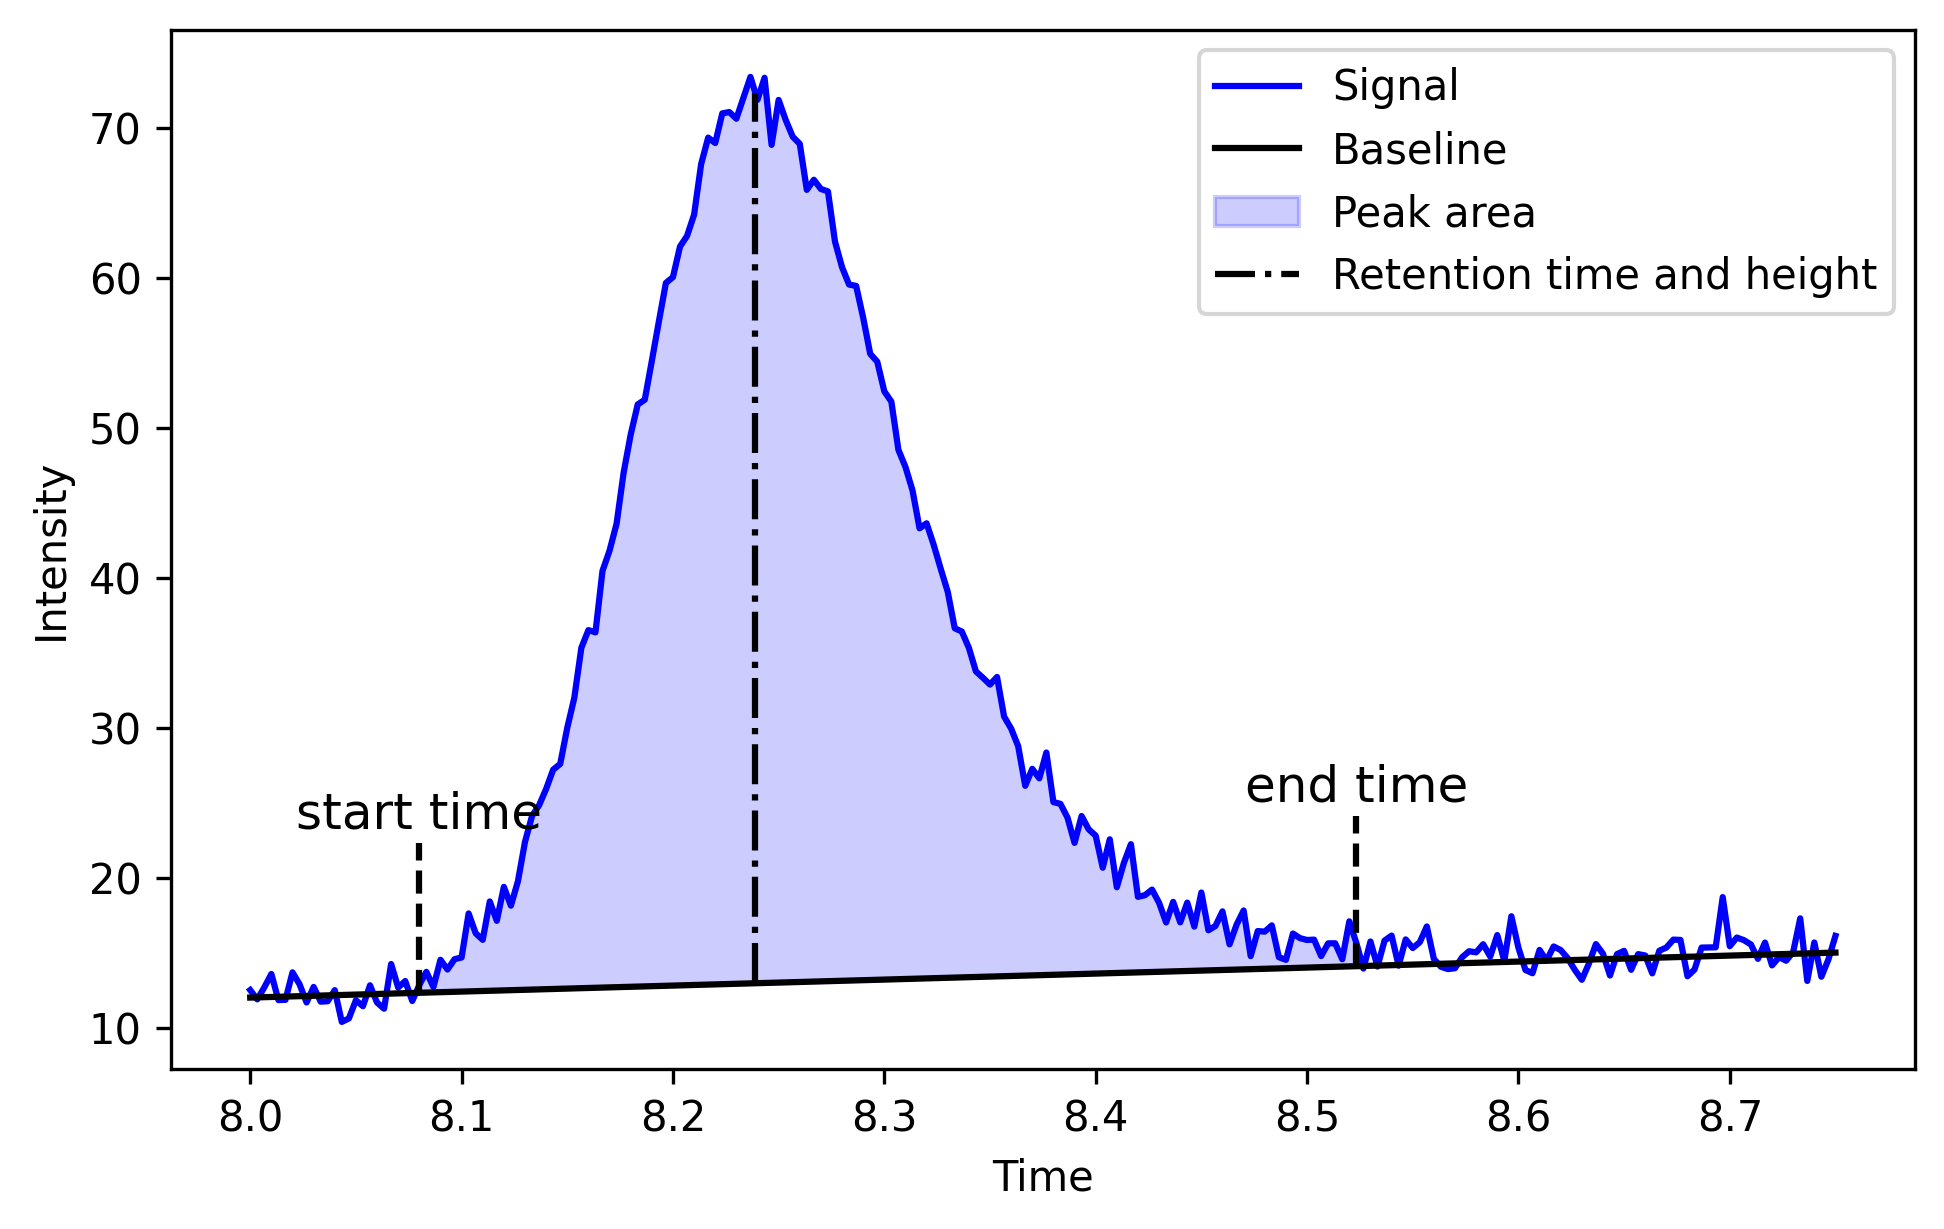
\includegraphics[width=\textwidth]{baseline_and_retention_time} % first figure itself
        \caption{Peak showing peak start and end times, retention time, and baseline.}\label{fig:times}
        \vfill
    \end{minipage}\hfill 
    \begin{minipage}[t]{0.45\textwidth}
        \centering
        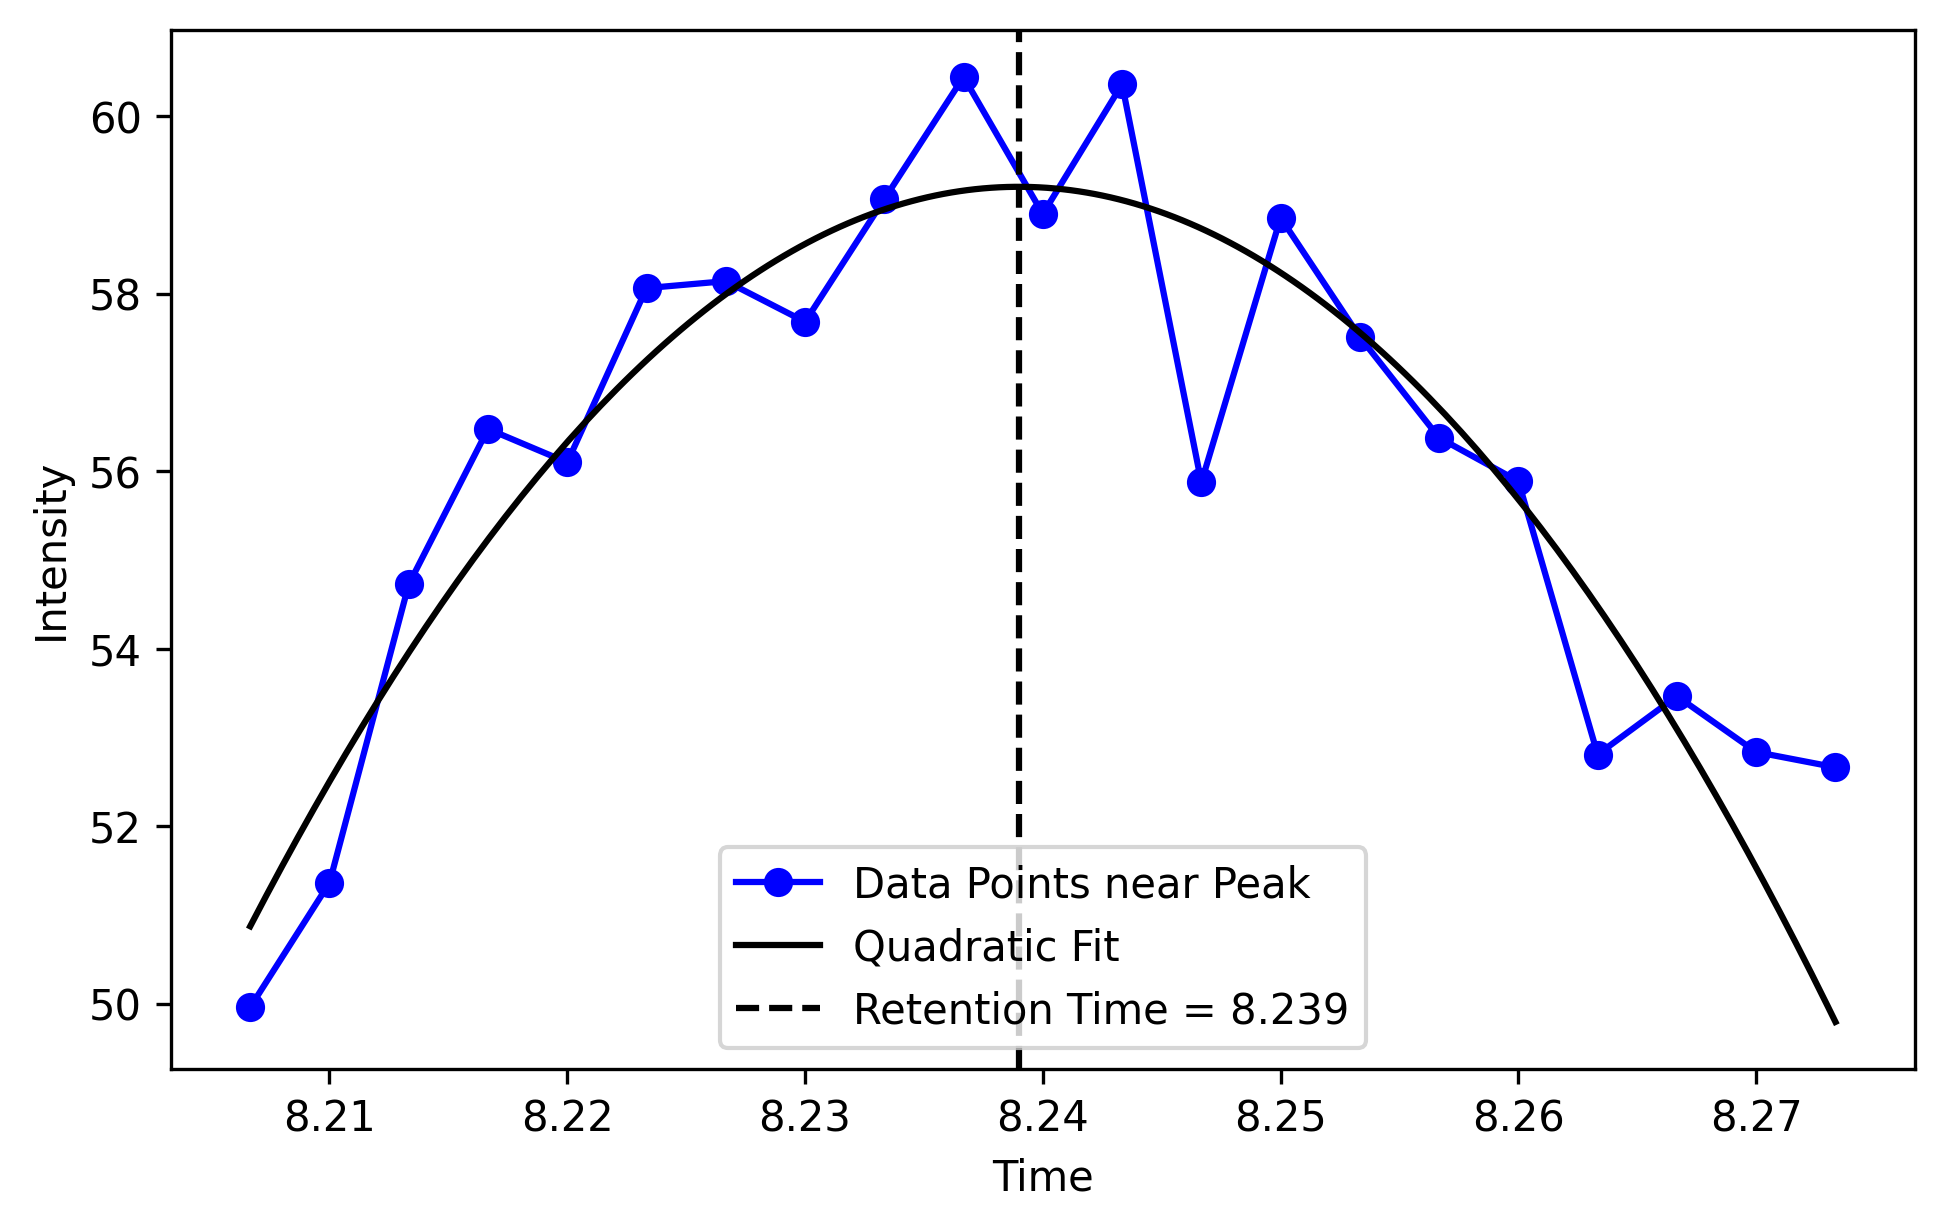
\includegraphics[width=\textwidth]{quadratic_fit} % second figure itself
        \caption{Peak apex showing quadratic fit at the top of the peak, and the calculated retention time.}\label{fig:quad-fit}
    \end{minipage}
\end{figure}

Peak start and end are determined by the peak detection algorithm. They are selected so the peaks may start and end at the same time, but no peaks may overlap. 

\dbtt{start\_time} and \dbtt{end\_time}: The start and end of the peak as determined by the detection algorithm in \ref{sec:detectionalg}, depicted in Figure {fig:times}. In the following peak parameters, start time is typically denoted $t_i$ (for initial time) and end time as $t_f$ (for final time). 

\dbtt{retention\_time}: The time at which a peak exhibits maximum height above baseline. To account for noise in the signal, the highest point in the raw signal is found, and a quadratic curve is fit to the series of time/signal points starts starting three points before the maximal signal and ending three after. The time  coordinate of the vertex of this quadratic is set to be the retention time, $t_R$. The signal coordinate of this vertex is set to be the peak height. 

\dbtt{start\_baseline}, \dbtt{end\_baseline}: The values of the baseline at the \dbtt{start\_time} and \dbtt{end\_time}, with the units of the signal.

\dbtt{retention\_baseline}: The baseline value at the retention time, as calculated by linear interpolation from the start and end times and start and end baseline values.

\dbtt{start\_signal} and \dbtt{end\_signal}: The start and end signal values, with the units of the signal.

\subsubsection{Type}


\subsubsection{Quantification}

\dbtt{area}: The area $A$ of the peak under the raw signal and above the baseline:$$A = \int_{t_i}^{t_f} f(t) \approx \sum_{k=u}^k f(t_k) \Delta t,$$
where $f(t)$ is the baseline-corrected signal. Units are in $\text{signal} \cdot \text{time}$; for UV-Vis, the units are $\text{mAU} \cdot \text{min}$.

\dbtt{relative\_area}: The percentage of area of the peak relative to the summed area of all peaks; that is, if there are $n$ peaks, peak $i$ has relative area $$A_{\text{rel}} = 100\% \cdot \frac{A_i}{\sum\limits_{k=1}^n A_k}$$
with units of percent.

\dbtt{capillary\_electrophoresis\_area}: Equal to $A/t_R$, the capillary electrophoresis area is the area adjusted for migration (retention) time in capillary electrophoresis to compensate for changes in migration time between runs
 
\dbtt{height}: The maximal height $h$ of the above the baseline at the retention time $t_R$. This height is calculated using a quadratic approximation to the apex of the peak; see the \dbtt{retention\_time} entry in section \ref{sec:times}. Height units are the units of the signal. 

\dbtt{relative\_height}\label{def:height} The percentage of the peak's height above baseline relative to the summed heights above baseline for all peaks: $$h_{\text{rel}} = 100\% \cdot \frac{h_i}{\sum\limits_{k=1}^n h_k}$$
with units of percent.
 


\subsubsection{Widths}
When possible, peak widths are calculated based on actual signal data, determining at what time a signal crosses a height threshold to the left and right of the retention time. For peaks that are not baseline resolved, it may be necessary to use extended peak calculations to estimate peak widths. 

\dbtt{width\_50\_<left,right,full>}: The left, right, and full peak width of the peak at 50\% height. 

\dbtt{width\_10\_<left,right,full>}: The left, right, and full peak width of the peak at 10\% height. 

\dbtt{width\_50\_<left,right,full>}: The left, right, and full peak width of the peak at 5\% height. 

\dbtt{width\_4\_sigma\_<left,right,full>}: The left, right, and full peak width of the peak at $4\sigma \approx 13.4\%$ height. 

\dbtt{width\_5\_sigma\_<left,right,full>}: The left, right, and full peak width of the peak at $5\sigma \approx 4.4\%$ height. 

\dbtt{width\_baseline\_<left,right,full>}: The left and right points of inflection of the fitted exponentially-modified gaussian are first calculated. The slopes at these two points are then calculated, and the lines with this slope going through these two points are extended to the baseline. The left, right, and full baseline widths are determined based on where these slope lines intersect the baseline, as well as a vertical line at $t_R$. 

\dbtt{extended\_width\_calculation}: an array of the string value names for which extended peak width calculations were needed to calculate, as opposed to using raw signal values.

\subsubsection{Statistical Moments}\label{sec:moments}
Statistical moments quantify aspects of the peak shape. For the calculation of peak shapes, the function $f(t)$ is the baseline-corrected signal, which is equal to the raw signal after subtraction of the baseline. For the calculation of moments, the absolute value of this function is use to avoid negative moments, which can lead to runtime errors when calculating higher moments. This will result in differences between \btt{moment 0} and the \btt{area} for smaller peaks when noise levels cause the signal to drop below the baseline. 

\dbtt{moment\_0}: Equal to peak area. For peak start time $t_i$ and peak end $t_f$ and baseline-corrected signal $f(t)$,  
$$ \mu_0 = \int_{t_i}^{t_f} |f(t)| dt \approx \sum_{k = i}^{f} |f(t_k)| \Delta t.$$ 
Units are equal to the signal value multiplies by time in minutes, e.g. $\text{mAU}\cdot \text{min}$.

\dbtt{moment\_1}: Average retention time. For peak start time $t_i$ and peak end $t_f$ and baseline-corrected signal $f(t)$,  
$$ \mu_2 = \frac{1}{\mu_0} \int_{t_i}^{t_f} t\cdot |f(t)| dt \approx \sum_{k = i}^{f} t_k \cdot |f(t_k)| \Delta t$$ 
Units are in minutes.

\dbtt{moment\_2}: Retention time variance. For peak start time $t_i$ and peak end $t_f$ and baseline-corrected signal $f(t)$,  
\begin{align*}
\mu_2 &= \frac{1}{\mu_0} \int_{t_i}^{t_f} (t - \mu_1 )^2 \cdot |f(t)| dt \approx \sum_{k = i}^{f} (t_k - \mu_1 )^2 \cdot |f(t_k)| \Delta t
\end{align*}
Units are in $\text{min}^2$.

\dbtt{standard\_deviation}: Retention time standard deviation. Standard deviation $\sigma = \sqrt{\mu_2}$. Units are in $\text{min}$.

\dbtt{moment\_3}: Third central moment of retention time. For peak start time $t_i$ and peak end $t_f$ and baseline-corrected signal $f(t)$,  
\begin{align*}
\mu_3 &= \frac{1}{\mu_0} \int_{t_i}^{t_f} (t - \mu_1 )^3 \cdot |f(t)| dt \approx \frac{1}{\mu_0}\sum_{k = i}^{f} (t_k - \mu_1 )^3 \cdot |f(t_k)| \Delta t
\end{align*}
Units are in $\text{min}^3$.

\dbtt{moment\_3\_normalized}: Third normalized moment of retention time, or statistical skewness (not to be confused with USP skewness). For peak start time $t_i$ and peak end $t_f$ and baseline-corrected signal $f(t)$,  
\begin{align*}
\tilde{\mu}_3 &= \frac{1}{\mu_0\cdot\mu_2^{3/2}} \int_{t_i}^{t_f} (t - \mu_1 )^3 \cdot |f(t)| dt \approx \frac{1}{\mu_0\cdot\mu_2^{3/2}}\sum_{k = i}^{f} (t_k - \mu_1 )^3 \cdot |f(t_k)| \Delta t
\end{align*}
The normalized moment is unitless.

\dbtt{moment\_4}: Fourth central moment of retention time. For peak start time $t_i$ and peak end $t_f$ and baseline-corrected signal $f(t)$,  
\begin{align*}
\mu_4 &= \frac{1}{\mu_0} \int_{t_i}^{t_f} (t - \mu_1 )^4 \cdot |f(t)| dt \approx \frac{1}{\mu_0}\sum_{k = i}^{f} (t_k - \mu_1 )^4 \cdot |f(t_k)| \Delta t
\end{align*}
Units are in $\text{min}^4$.

\dbtt{moment\_4\_normalized}: Fourth central moment of retention time, or kurtosis. For peak start time $t_i$ and peak end $t_f$ and baseline-corrected signal $f(t)$,  
\begin{align*}
\tilde{\mu}_4 &= \frac{1}{\mu_0\cdot \mu_2^2} \int_{t_i}^{t_f} (t - \mu_1 )^4 \cdot |f(t)| dt \approx \frac{1}{\mu_0\cdot \mu_2^2}\sum_{k = i}^{f} (t_k - \mu_1 )^4 \cdot |f(t_k)| \Delta t
\end{align*}
The normalized moment is unitless.

\subsubsection{Asymmetry}
Asymmetry provides a measure for how much a peak is tailing or fronting. This metric may be used to monitor column quality. For the USP/EP and AIA definitions, as well as skewness, ideal peaks have a value near 1, while peaks less than 1 signify a fronting peak, and values greater than 1 signify a tailing peak. Unless otherwise stated in a test or assay, the USP standard requires \dbtt{asymmetry\_USP} to fall between 0.8 and 1.8 if the peak is to be used for quantification. 

For statistical asymmetry, ideal peaks are scattered around 0; this value is negative for fronting peaks and positive for tailing peaks.\\

\dbtt{asymmetry\_USP}: US Pharmacopoeia calculation for asymmetry; this is identical to the European Pharmacopoeia (EP) and Japanese Pharmacopoeia (JP) definition: $$ A = \frac{RW_{5\%} + LW_{5\%}}{2 \cdot LW_{5\%}} = \frac{W_{5\%}}{2 \cdot LW_{5\%}}$$ for 5\% left, right and full widths, $LW_{5\%}$, $RW_{5\%}$, and $W_{5\%}$. This value is undefined if these widths cannot be calculated. This value is also sometimes called the \btt{tailing factor} or \btt{asymmetry factor}.

\dbtt{asymmetry\_AIA}: AIA calculation for asymmetry: $$ A = \frac{RW_{10\%}}{LW_{10\%}} $$ for 10\% left and right widths, $LW_{10\%}$ and $RW_{10\%}$. This value is undefined if these widths cannot be calculated.

\dbtt{asymmetry\_statistical}: Calculation of asymmetry using moments: $$ A = \frac{\mu_1 - t_R}{\sqrt{\mu_2}} $$ for first and second statistical moments $\mu_1$ and $\mu_2$ (see \ref{sec:moments}), and retention time $t_R$.

\dbtt{skewness}: Metric similar to asymmetry. Not to be confused with statistical skewness, which is equal to the third normalized moment of retention time, $\tilde{\mu_3}$, as defined in \ref{sec:moments}. This measure of skewness is defined as: 
$$ S = \frac{RW_{10\%} + LW_{10\%}}{2 \cdot LW_{10\%}}$$
for 10\% left and right widths, $LW_{10\%}$ and $RW_{10\%}$. This value is undefined if these widths cannot be calculated.

\subsubsection{Resolution}
Resolution measures how well two peaks are separated, using the width of two peaks and the distance in time between them. Resolution is always defined with regard to a reference peak; a peak cannot reference itself. The module uses the USP, EP/JP, and statistical moments methods each for up to five different reference peaks, where the string value in parenthesis is replaces \dbtt{<type>}  in the resolution field name: 
\begin{enumerate}
\item previous main peak (\dbtt{previous\_main}): the previous quantified peak
\item next main peak (\dbtt{next\_main}): the next quantified peak
\item previous named peak (\dbtt{previous\_named}): the previous peak with a name that is not equal to \texttt{None}, \texttt{""}, or \texttt{"unknown"}.
\item next named peak (\dbtt{next\_named}): the next peak with a name that is not equal to \texttt{None}, \texttt{""}, or \texttt{"unknown"}.
\item specified reference peak (\dbtt{reference}): a peak specified by name in the processing method (see section \ref{sec:procmeth}).
\end{enumerate}

\dbtt{resolution\_ep\_<type>}: European Pharmacopoeia calculation for resolution $R$, where for a reference peak \textit{ref}, $$ R = 1.18 \left| \frac{t_{\textit{ref}} - t_R}{W_{50\%, \textit{ref}}+W_{50\%, R}} \right|$$

\dbtt{resolution\_usp\_<type>}: US Pharmacopoeia calculation for resolution $R$, where for a reference peak \textit{ref}, $$ R = 2 \left| \frac{t_{\textit{ref}} - t_R}{\text{BW}_{\textit{ref}}+\text{BW}_R} \right|$$

\dbtt{resolution\_statistical\_<type>}: Statistical moments calculation for resolution $R$, where for a reference peak \textit{ref}, $$ R = \left| \frac{t_{\textit{ref}} - t_R}{2 \left(\sqrt{\mu_{2,\textit{ref}}} + \sqrt{\mu_2}\right)} \right|$$

\dbtt{signal\_to\_noise}:

\subsubsection{Theoretical Plates}
\dbtt{plates\_EP}: European Pharmacopoeia calculation for theoretical plates TP, where for retention time $t_R$ and 50\% width $W_{50\%}$, $$\text{TP} = 5.54 \left( \frac{t_R}{W_{50\%}}\right)^2$$

\dbtt{plates\_USP}: US Pharmacopoeia calculation for theoretical plates TP, where for retention time $t_R$ and baseline width BW, $$\text{TP} = 16 \left( \frac{t_R}{\text{BW}}\right)^2$$

\dbtt{plates\_statistical}: Statistical Moments calculation for theoretical plates TP, where for retention time $t_R$ and second statistical moment $\mu_2$, $$\text{TP} = \frac{t_R^2}{\mu_2}$$ 


\section{Samples}


\subsection{Sample Creation}

\subsubsection{Product Stability}

\subsubsection{Reaction Optimization}

\subsection{Samples JSON}

\printbibliography[heading=bibintoc]


\appendix
\appendixpage
\addappheadtotoc
\section{Future Implementation}
Future iterations of this module will include (in no particular order):
\begin{itemize}
\item A method to allow for different column types to produce different elution profiles
\item Enablement of pH-dependent phenomena, e.g. peak broadening and change in retention time, based on buffer pH and compound pK\textsubscript{a} and pK\textsubscript{b} values.
\item Improved scientific model for estimating elution times based on solvent, column, and compound properties
\item Additional spectra types
\begin{itemize}
\item 3D UV-Vis
\item CAD/ELSD
\item Fluorescence
\item MS
\end{itemize}

\end{itemize}

\section{Classes}
\lstset{language=Python}
\lstset{style=pythonstyle}
\subsection{\btt{Injection}}

\subsubsection{Instantiation}
\begin{lstlisting}
Injection(
    sample: Sample,
    method: InstrumentMethod,
    processing_method: ProcessingMethod,
    sequence: Sequence,
    system: System,
    user: str | None = "admin",
    injection_time: datetime.datetime | None = None,
)
\end{lstlisting}
\subsubsection{Methods}

\subsubsection{Dictionary Keywords}

\subsection{\btt{System}}

\subsection{\btt{Column}}

\subsection{\btt{InstrumentMethod}}

\subsection{\btt{ProcessingMethod}}

\subsubsection{Instantiation}

\subsubsection{Methods}

\subsubsection{Dictionary Keywords}

\subsection{\btt{Compound}}
\subsection{\btt{Sample}}
\subsection{\btt{Chromatogram}}
\subsection{\btt{PeakFinder}}
\subsection{\btt{PeakList}}
\subsection{\btt{Peak}}

\section{Example Input JSON}
\lstset{style=jsonstyle}
\subsection{System}
\begin{lstlisting}
{
    "name": "Curie",
    "software": "Chromeleon",
    "manufacturer": "ThermoFisher",
    "modules": [
        {
            "name": "Sampler",
            "manufacturer": "Thermo Fisher Scientific Inc.",
            "type": "Autosampler",
            "detector_type": null,
            "part_number": "ACC-3000T",
            "serial_number": "23056882"
        },
        {
            "name": "PumpModule.Pump",
            "manufacturer": "Thermo Fisher Scientific Inc.",
            "type": "Pump",
            "detector_type": null,
            "part_number": "LPG-3400SD",
            "serial_number": "96014241"
        },
        {
            "name": "UV",
            "manufacturer": "Thermo Fisher Scientific Inc.",
            "type": "Detector",
            "detector_type": "UV-Vis",
            "part_number": "DAD-3000RS",
            "serial_number": "54202953",
            "firmware_version": "1.10.0",
            "driver_version": "7.3.2.10759"
        }
    ],
    "column": {}
    },
    "system_retention_time_offset": 0.021
}
\end{lstlisting}
\subsection{Column}
\begin{lstlisting}
{
    "inner_diameter": {
        "value": 10,
        "unit": "mm"
    },
    "length": {
        "value": 150,
        "unit": "mm"
    },
    "type": "C18",
    "serial_number": "1995032",
    "injection_count": 0,
    "particle_size": {
        "value": 5,
        "unit": "um"
    }
}
\end{lstlisting}

\subsection{Instrument Method}
\begin{lstlisting}
{
    "name": "column_quality_check",
    "run_time": 8,
    "mobile_phases": [
        {
            "name": "water",
            "id": "A"
        },
        {
            "name": "THF",
            "id": "B"
        },
        {
            "name": "methanol",
            "id": "C"
        },
        {
            "name": "acetonitrile",
            "id": "D"
        }
    ],
    "mobile_phase_gradient_steps": [
        {
            "time": 0.0,
            "flow": 5.0,
            "percent_a": 100.0,
            "percent_b": 0.0,
            "percent_c": 0.0,
            "percent_d": 0.0,
            "curve": 5
        },
        {
            "time": 8.0,
            "flow": 5.0,
            "percent_a": 85.0,
            "percent_b": 15.0,
            "percent_c": 0.0,
            "percent_d": 0.0,
            "curve": 5
        }
    ],
    "detection": {
        "uv_vis_parameters": [
            {
                "name": "UV_VIS_1",
                "wavelength": 250,
                "bandwidth": 4
            },
            {
                "name": "UV_VIS_2",
                "wavelength": 270,
                "bandwidth": 4
            }
        ]
    },
    "creation": {
        "computer": "CHROMELEON2",
        "comment": null,
        "time": "2020-08-31T12:18:06.01Z",
        "user": "cmadmin",
        "data_vault_name": "CHROMELEON2/ChromeleonLocal"
    },
    "last_update": {
        "computer": "CHROMELEON2",
        "comment": null,
        "time": "2020-08-31T12:24:33.75Z",
        "user": "cmadmin",
        "data_vault_name": "CHROMELEON2/ChromeleonLocal"
    },
    "sample_introduction": {
        "dilution_factor": 1.0,
        "injection_volume": 20.0,
        "weight": 1.0,
        "internal_standard_amount": 1.0,
        "autodilution_ratio": 0.0
    }
}
\end{lstlisting}

\subsection{Processing Method}
\begin{lstlisting}
{
    "name": "column performance test",
    "detection_parameters": {
        "background_noise_range": {
            "minimum": 0,
            "maximum": 250
        },
        "noise_threshold_multiplier": 10,
        "peak_limit": 5,
        "minimum_height": {
            "type": "baseline_noise_multiplier",
            "value": 10
        },
        "minimum_area": 0.3
    },
    "resolution_reference": "TS-8391",
    "peak_identification": [
        {
            "min_time": 2.0,
            "max_time": 2.5,
            "method": "largest",
            "name": "TS-8391"
        },
        {
            "min_time": 3.6,
            "max_time": 4.1,
            "method": "largest",
            "name": "klimavizinib",
            "calibration": {
                "type": "linear",
                "amount_unit": "umol/mL",
                "points": [
                    {
                        "area": 101.2,
                        "amount": 2.5
                    },
                    {
                        "area": 99.2,
                        "amount": 2.5
                    },
                    {
                        "area": 1002,
                        "amount": 25
                    },
                    {
                        "area": 987.4,
                        "amount": 25
                    },
                    {
                        "area": 10,
                        "amount": 0.25
                    },
                    {
                        "area": 9.3,
                        "amount": 0.25
                    },
                    {
                        "area": 9.2,
                        "amount": 0.25
                    },
                    {
                        "area": 0.913,
                        "amount": 0.025
                    },
                    {
                        "area": 1.01,
                        "amount": 0.025
                    },
                    {
                        "area": 4.989,
                        "amount": 0.125
                    },
                    {
                        "area": 5.12,
                        "amount": 0.125
                    }
                ]
            }
        },
        {
            "min_time": 5.9,
            "max_time": 6.4,
            "method": "largest",
            "name": "caffeine"
        }
    ]
}
\end{lstlisting}

\section{Adding to the Compound Library}
The compound library is stored in the 


%\end{multicols}


\end{document}
